\documentclass[11pt]{article}
\usepackage[margin=1in,footskip=0.25in]{geometry}
\usepackage{hyperref}
\usepackage{graphicx}
\usepackage[T1]{fontenc}
\usepackage{listings}
\usepackage{xcolor}
 
\definecolor{codegreen}{rgb}{0,0.6,0}
\definecolor{codegray}{rgb}{0.5,0.5,0.5}
\definecolor{codepurple}{rgb}{0.58,0,0.82}
\definecolor{backcolour}{rgb}{0.95,0.95,0.92}
 
\lstdefinestyle{mystyle}{
    backgroundcolor=\color{backcolour},   
    commentstyle=\color{codegreen},
    keywordstyle=\color{magenta},
    numberstyle=\tiny\color{codegray},
    stringstyle=\color{codepurple},
    basicstyle=\ttfamily\footnotesize,
    breakatwhitespace=false,         
    breaklines=true,                 
    captionpos=b,                    
    keepspaces=true,                 
    numbers=left,                    
    numbersep=5pt,                  
    showspaces=false,                
    showstringspaces=false,
    showtabs=false,                  
    tabsize=2
}
 
\lstset{style=mystyle}

\usepackage{amsthm}
\usepackage{amsmath}
\usepackage{graphicx}
\usepackage{multicol, latexsym, amssymb}
\usepackage{blindtext}
\usepackage{subcaption}
\usepackage{caption}
\usepackage{algorithm}
\usepackage{algorithmic}

\usepackage{tabu}

\begin{document}

\title{
{\textbf{CS591S1 Homework 1: Attacks and DP Basics}}
}
\author{Jiawen Liu\\
Collaborators: none.}

\date{}
\maketitle

\section{Problem 1}

\begin{enumerate}
	\item The only input to the attacker is a (the vector of noisy counters).
\begin{itemize}
\item \textbf{Algorithm Description}
%
%
\begin{algorithm}
\caption{Reconstruction Attack without Extra Information}
\label{alg_p1-1}
\begin{algorithmic}
\REQUIRE The observed results $a$ from query.
\STATE {\bf Initialize $c = a$}, as the reconstructed counter . 
\STATE  {\bf for}\ $i\in [a.length]$\ {\bf do}.  
\STATE \qquad {\bf let} 
	$s = a[i] - c[i - 1]$ 
	\COMMENT {be the noised $i_{th}$ item in data set.}
\STATE \qquad {\bf If} $s > 1$  {\bf do}.
		$c[i] = a[i] - 1$
		\COMMENT {the correct counter at position i must be a[i] - 1.}
\STATE \qquad {\bf Elif} $s < 0$  {\bf do}.
\STATE \qquad \qquad 
		{\bf let} $j = i$
\STATE \qquad \qquad {\bf While} 
		$j - 1 > 0 \land c[j] < c[j - 1]$  {\bf do}.
		$j = j - 1$;
		$c[j] = c[j] - 1$
\STATE	\COMMENT {the correct counter at position i must be a[i] and decrease all the previous abnormal items by 1}

\RETURN $s_i = c_{i} - c_{i - 1}$ {\bf for}\ $i\in [a.length]$.
\end{algorithmic}
\end{algorithm}
%
\item \textbf{Experimental Results Plotting}
%
Figure \ref{fig-p1-1}
%
\begin{figure}[h]
    \centering
    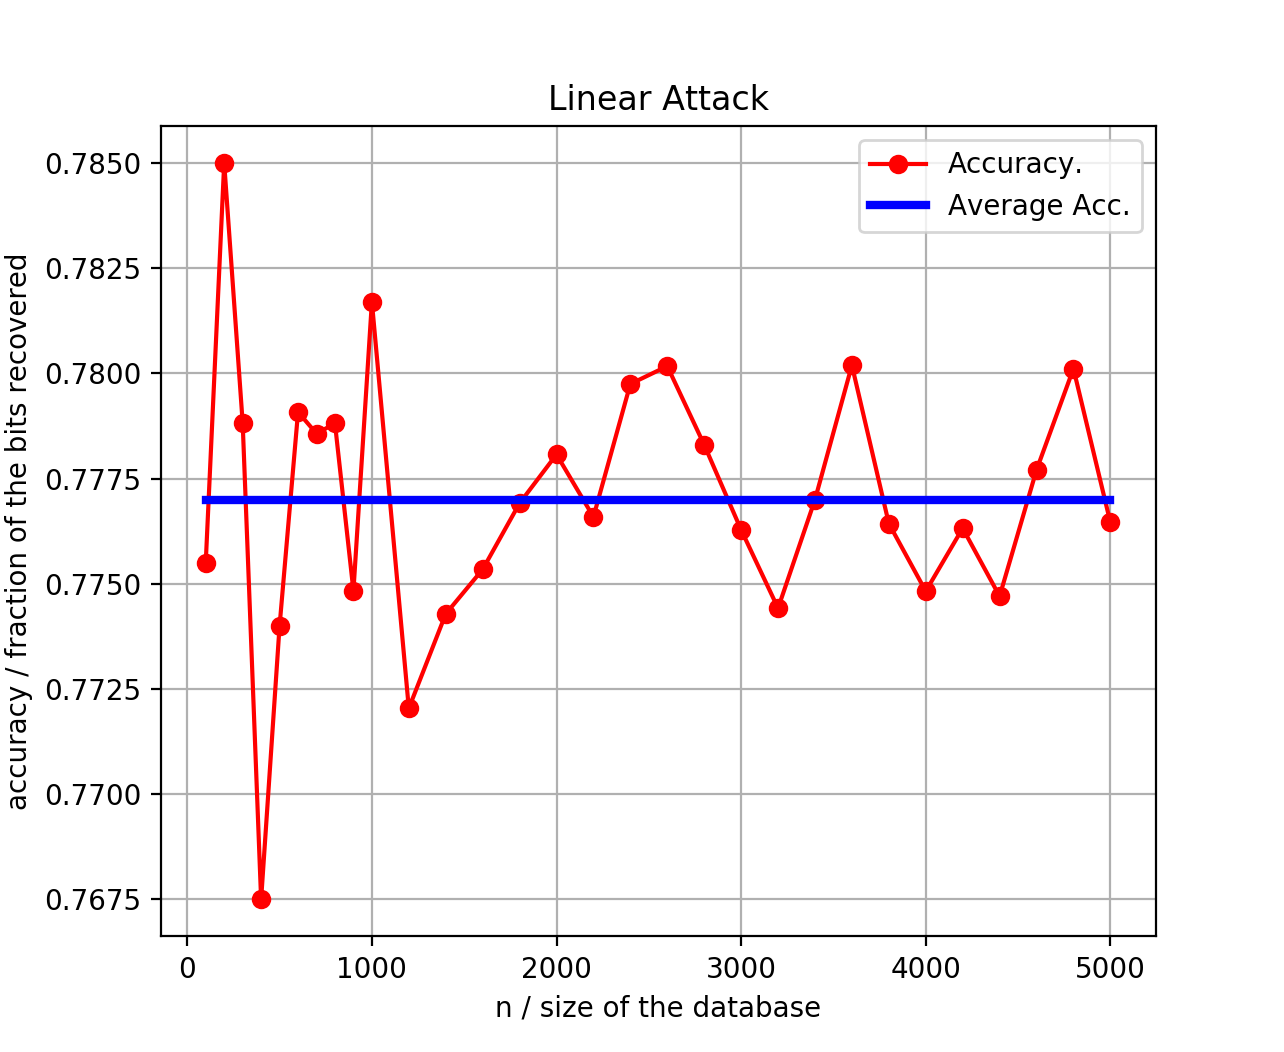
\includegraphics[width=0.6\textwidth]{p1-1.eps}
    \caption{P1 - 1 : accuracy of recontruction attack without aux information}
    \label{fig-p1-1}
\end{figure}
%
\item \textbf{Results Discussion}
%

%
The average accuracy is 0.7775 from the Alg. \ref{alg_p1-1}, which is higher than 0.75.
%
\\%
I also got different results form some attempts before I achieved this result:
%
\\
%
\textbf{attempt 1.}
I first tried the naive method in Alg. \ref{alg_p1-1-2}, which only achieved standard 0.75 accuracy on average.
%
\begin{algorithm}
\caption{Naive Reconstruction Attack without Extra Information}
\label{alg_p1-1-2}
\begin{algorithmic}
\REQUIRE The observed results $a$ from query.
\STATE {\bf Initialize vector s: $s[i] = a[i] - a[i - 1]$} 
\COMMENT {as the reconstructed dataset.} 
\STATE  {\bf for}\ $i\in [a.length]$\ {\bf do}.  
\STATE \qquad {\bf If} $s > 1$  {\bf do}.
    $s[i] = 1$
\STATE \qquad {\bf Elif} $s < 0$  {\bf do}.
	$s[i] = 0$
\RETURN $s$.
\end{algorithmic}
\end{algorithm}
%
\\
%
\textbf{Attempt 2.}
Then I tried the minimizing error method from class in Alg. \ref{alg_p1-1-3}, which achieved a better accuracy but is inefficient. 
I'm able to achieve higher accuracy for small size data base with large iteration number $T$.
However,
I cannot even get the results for $n = 1000$ in resonable time.
%
\begin{algorithm}
\caption{Minimizing Error Reconstruction Attack without Extra Information}
\label{alg_p1-1-3}
\begin{algorithmic}
\REQUIRE The observed results $a$ from query, the number of iteration $T$, the query result release mechanism $M$.
\STATE {\bf Initialize dataset s, error e, $s[i] \leftarrow \{0, 1\}$, $e = Inf$}. 
\STATE  {\bf for}\ $i\in [T]$\ {\bf do}.  
\STATE \qquad sample a new data set $s'$
\STATE \qquad $e' = sum(a - M(s'))$;
\STATE \qquad  {\bf If}\ $ e' < e$\ {\bf do}. s = s'; e = e'
\RETURN $s$.
\end{algorithmic}
\end{algorithm}
%
\\
%
\textbf{Attempt 3, Alg. \ref{alg_p1-1}.}
%
Then I go back to the Alg. \ref{alg_p1-1-2} and made some improvements in it.
\begin{itemize}
	\item Instead of recovering the data base directly, I firstly recovered the counter.
	% 
	\item In the situation where $a[i] - a[i - 1] < 0$, instead of just setting $s[i]$ be $0$, I went back and retraced the previous result.
\end{itemize}
These two steps improved the accuracy from the naive method.

\item \textbf{Code Documentation}
%
See Appendix \ref{code-p1-1}.
%
\item{Repository Link}

\url{ https://github.com/jiawenliu/CS591S1.git }
\end{itemize}

\item The attacker's inputs consist of a and the vector of guesses w.

	\begin{itemize}
	\item \textbf{Algorithm Description}
	%
	\begin{algorithm}
	\caption{Reconstruction Attack with Extra Information}
	\label{alg_p1-1}
	\begin{algorithmic}
	\REQUIRE The observed results $a$ from query, the guass $w$.
	\STATE {\bf Initialize $c = a$}, as the reconstructed counter. 
	\STATE {\bf Initialize $s' = [-1] * n$}, as the reconstructed data set where $n$ is the size of the dataset. 
	\STATE  {\bf for}\ $i\in [a.length]$\ {\bf do}.  
	\STATE \qquad {\bf let} 
		$s' = a[i] - c[i - 1]$ be the possible $j_{th}$ item in data set.
	\STATE \qquad {\bf If} $s' > 1$  {\bf do}.
			$c[i] = a[i] - 1$
	\STATE \qquad \qquad 
			{\bf let} $j = i$; $s[i] = 1$
	\STATE \qquad \qquad {\bf While} 
			$j - 1 \geq 0 \land c[j] > c[j - 1]$  {\bf do}.
			$j -= 1$
			$s[j] = 1$
			\COMMENT {the correct counter at position i must be a[i] - 1}
	\STATE \qquad {\bf Elif} $s' < 0$  {\bf do}.
	\STATE \qquad \qquad 
			{\bf let} $j = i$; $s[i] = 0$
	\STATE \qquad \qquad {\bf While} 
			$j - 1 > 0 \land c[j] < c[j - 1]$  {\bf do}.
			$j -= 1$
			$c[j] -= 1$
	\STATE	\COMMENT {the correct counter at position i must be a[i] and decrease the previous by 1 until their difference $\geq 0$}
	\STATE  {\bf for}\ $i\in [a.length]$\ {\bf do}.  
	\STATE \qquad {\bf If} $s[i] == -1$  {\bf do}.
			$s[i] = w[i]$
	\STATE	\COMMENT {If $s[i]$ is -1, means s[i] is uncertain, before we are using c[i] - c[i-1], right now we are using guess[i], which has higher accuracy}

	\RETURN $s$.
	\end{algorithmic}
	\end{algorithm}
	%
	\item \textbf{Experimental Results Plotting}
	%
	Figure \ref{fig-p1-2}
\begin{figure}[h]
    \centering
    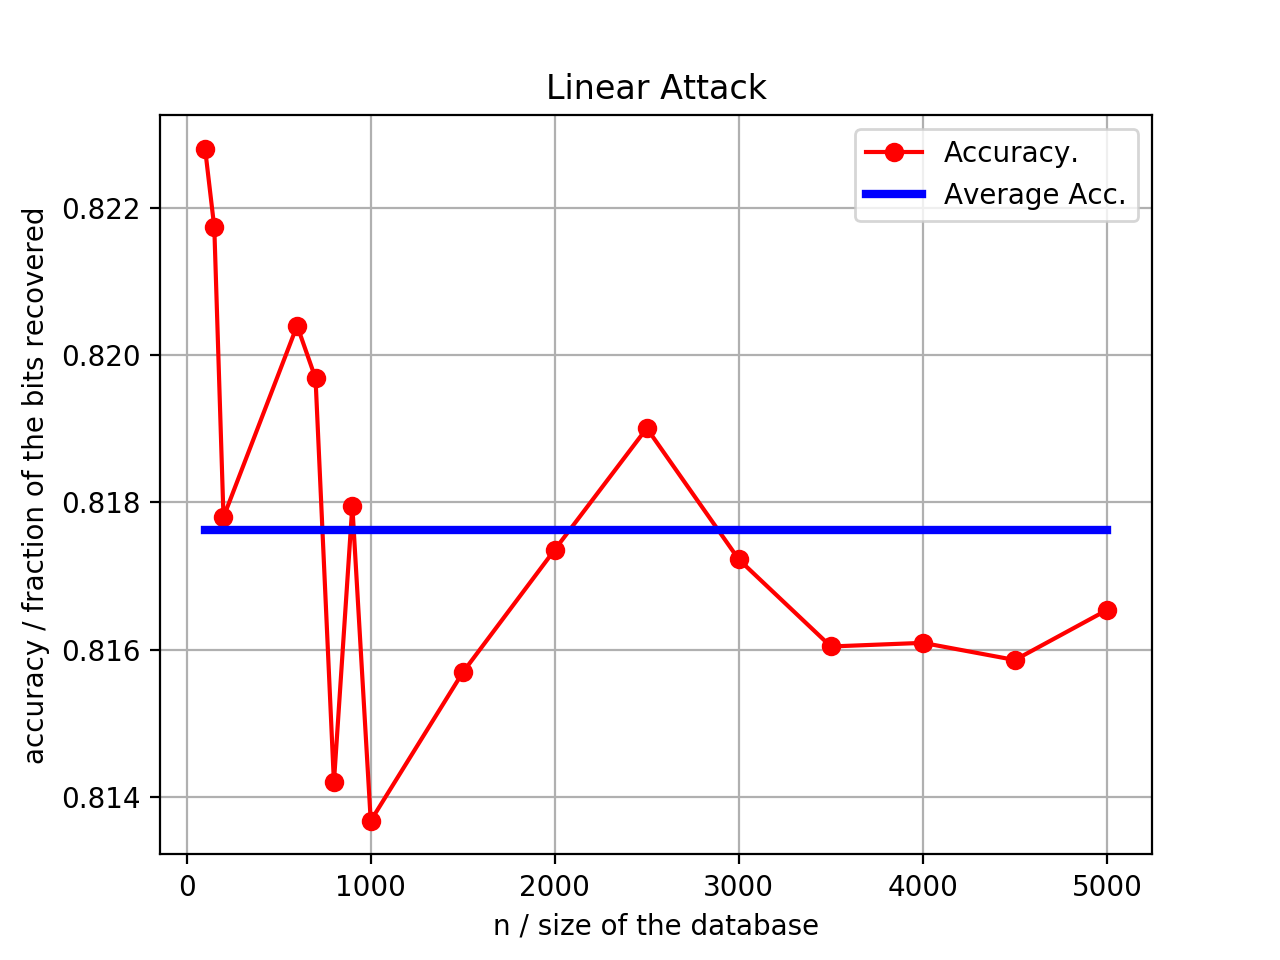
\includegraphics[width=0.6\textwidth]{p1-2.eps}
    \caption{P1 - 2 : accuracy of recontruction attack with aux information}
    \label{fig-p1-2}
\end{figure}	%
	\item \textbf{Results Discussion}
	%
	This one has higher accuracy than without using side information around $0.82$.

	Because when without side information, in the case of uncertainty, we can only guess without any help. The accuracy of random guess is $\frac{1}{2}$. But when we have the guess of accuracy $\frac{2}{3}$, we guess higher accuracy in the case of uncertainty. Then the accuracy will be improved.
	%
	\item \textbf{Code Documentation}
	%
	%
	The Code are exactly the same as code in previous part, except adding one function in Appendix \ref{code-p1-2}
	%
\end{itemize}
\end{enumerate}

\section{Problem 2}
\begin{enumerate}
\item
\begin{enumerate}
	\item[\textbf{(a)}]
	Given $X_i(j)$ sampled from $\{-1, 1\}$ i.i.d for $i = 1, \cdots, n$ and $j = 1, \cdots, d$, we have:
	\[
	\begin{array}{c}
	E(X_i(j)) = 0, ~ Var(X_i(j)) = 1\\
	E(\bar{X}(j)) = E(\frac{1}{n}\sum_i X_i(j)) = 0, 
	~ Var(\bar{X}(j)) = Var(\frac{1}{n}\sum_i X_i(j)) = \frac{1}{n}\\
	\end{array}
	\]
	Since $A = M(X) = \bar{X} + (Z(1), \cdots, Z(d))$ where $Z(j) \sim N(0, \sigma^2)$ independently from $X$, we have:
	\[
	E(A(j)) = 0, ~ Var(A(j)) = Var(\bar{X}(j) + Z(j)) = \frac{1}{n} + \sigma^2
	\]
	%
	Since $T_{out}$ is independently from $A$, we can conclude the expectation of $F(A, T_{out})$:
	\[
	E(F(A, T_{out})) = E(\sum_{j = 1}^{d}A(j) * T_{out}(j))
	= \sum_{j = 1}^{d} E(A(j) * T_{out}(j))
	= 0
	\]
	%
	and the standard deviation:
	\[
	\begin{array}{rl}
	& \sqrt{Var(F(A, T_{out}))}\\
	= & \sqrt{Var(\sum_{j = 1}^{d}A(j) * T_{out}(j))}\\
	= & \sqrt{\sum_{j = 1}^{d}Var(A(j) * T_{out}(j))}\\
	= & \sqrt{ \sum_{j = 1}^{d}Var(A(j)) * Var(T_{out}(j))
	+ Var(A(j))*E(T_{out}(j))^2 + E(A(j))^2 * Var(T_{out}(j))}\\
	= & \sqrt{d \big(\frac{1}{n} + \sigma^2\big)}
	\end{array}
	\]
	%
	\item[\textbf{(b)}]
	Since $T_{in}$ is sampled from $X$ which is not independently from $A$ anymore, we have following:
	\[
	\begin{array}{ccl}
	F(A, T_{in}) 
	& = & \sum_{j = 1}^{d}A(j) * T_{in}(j)\\
	& = & \sum_{j = 1}^{d}(\bar{X}(j) + Z(j)) * T_{in}(j)\\
	& = & \sum_{j = 1}^{d}(\frac{1}{n} \sum_{i = 1}^{n}X_i(j) + Z(j)) * T_{in}(j)\\
	& = & \sum_{j = 1}^{d}
	(\frac{1}{n}( \sum\limits_{i = 1\ldots n \land i \neq in}
	X_i(j) + Z(j))* T_{in}(j) + \frac{1}{n}T_{in}(j)^2)
	\end{array}
	\]
	%
	Let $A_{/T_{in}} = \frac{1}{n}( \sum\limits_{i = 1\ldots n \land i \neq in}
	X_i(j) + Z(j))$, we have:
	%
	\[
	E(A_{/T_{in}}) = 0, 
	~ Var(A_{/T_{in}}) = (\frac{n - 1}{n^2} + \sigma^2)
	\]
	%
	So we have the expectation of $F(A, T_{in})$ as:
	%
	\[
	E(F(A, T_{in})) 
	= \sum_{j = 1}^{d}
	E((A_{/T_{in}} * T_{in}(j) + \frac{1}{n}T_{in}(j)^2))
	= \frac{d}{n}
	\]
	%
	and variance of $F(A, T_{in})$ as:
	%
	\[
	\begin{array}{ccl}
	Var(F(A, T_{in})) 
	& = & \sum_{j = 1}^{d}
	Var((A_{/T_{in}} * T_{in}(j) + \frac{1}{n}T_{in}(j)^2))\\
	& = & \sum_{j = 1}^{d}
	Var((A_{/T_{in}} * T_{in}(j))\\
	& = & d(\frac{n - 1}{n^2} + \sigma^2)
	\end{array}
	\]
	%
	The standard deviation is the square root of variance, i.e., $\sqrt{d(\frac{n - 1}{n^2} + \sigma^2)}$.
	%
	\item[\textbf{(c)}]
	\[
	d = 
	\bigg(\sqrt{\big(n + n^2\sigma^2\big)} 
	+ \sqrt{\big(n - 1 + n^2\sigma^2\big)} \bigg)^2
	\]
	%
	\begin{itemize}
		\item $\sigma = 0.1$
		\[
		d = 
		\bigg(\sqrt{\big(n + 0.01n^2\big)} 
		+ \sqrt{\big(n - 1 + 0.01n^2\big)} \bigg)^2
		\]
		%
		\item $\sigma = 1/n$
		\[
		d = 
		\bigg(\sqrt{\big(n + 1\big)} 
		+ \sqrt{\big(n\big)} \bigg)^2
		\]
		%
		\item $\sigma = 1/\sqrt{n}$
		\[
		d = \big(\sqrt{2n} 
		+ \sqrt{2n - 1} \big)^2
		\]
	\end{itemize}
\end{enumerate}

\item
\begin{enumerate}
	\item[\textbf{(a)}]
	%
	\begin{itemize}
		\item \textbf{Algorithms Description}
		%
		The Alg. \ref{alg_p2-2a}
		%
		\begin{algorithm}
		\caption{Inference Attack with Gaussi Mechanism}
		\label{alg_p2-2a}
		\begin{algorithmic}
		\REQUIRE The row and column \# of data base $d, n$, the parameter $\sigma$ for Guassi mechanism.
		\STATE {\bf Sample $d_{in}, d_{out} \leftarrow \{-1, 1\}^{d \times n}$}. 
		\STATE {\bf let query}\ $q(d) = map(sum, d.transpose)/n$
		\STATE {\bf let}\ $A = q(d_{in}) + [z_i \leftarrow N(0, \sigma) for\ i \in [d]]$
		\STATE {\bf let}\ 
		$score_{in}, score_{out} = A \dot d_{in}.transpose, A \dot d_{out}.transpose$

		\STATE	\COMMENT {the F score for each row in dataset in and dataset out.}
		
		\STATE {\bf let}\ 
		$c = $ Counting how many items in $score_{in}$ greater than all items in $score_{out}$.
		
		\STATE {\bf let}\  $p = c / n$

		\RETURN True positive $p$
		\end{algorithmic}
		\end{algorithm}
		%
		\item \textbf{Experimental Results Plotting}
		Figure \ref{fig-p2-2a}

		\begin{figure*}[t!]
		    \centering
		    \begin{subfigure}[t]{0.5\textwidth}
		        \centering
		        \includegraphics[width=\textwidth]{p2-gauss-1.eps}
		        \caption{$\sigma = 0.01$}
		    \end{subfigure}%
		    ~ 
		    \begin{subfigure}[t]{0.5\textwidth}
		        \centering
		        \includegraphics[width=\textwidth]{p2-gauss-2.eps}
		        \caption{$\sigma = 1/3$}
		    \end{subfigure}
		    \caption{P2 : Gaussian mechanism}
		    \label{fig-p2-2a}
		\end{figure*}
%
		\item \textbf{Results Discussion}
		%
		Repeating the Algorithm. \ref{alg_p2-2a}, we get the results poltted in Fig. \ref{fig-p2-2a}. 
		%
		\\
		%
		{\bf The Fig. \ref{fig-p2-2a}(a)} shows the True positive rate with guassi noise parameter $\sigma = 0.01$. We can see the accuracy achieved $1.0$ when data base columns number is $2000$. Actually already achieved $0.92$ when column number greater than $800$.
		%
		\\
		%
		{\bf The Fig. \ref{fig-p2-2a}(b)} shows the True positive rate with guassi noise parameter $\sigma = 1/3$. We can see the accuracy only achieved $0.38$ when data base columns number is $2000$. Even though the column number increase up to $5000$, accuracy only get to around $0.68$.
		%
		\\
		From the two comparison, we can tell the smaller the parameter $\sigma$ is, the more accuracy it is. This is consistent with our intuition that the smaller noise results in more accuracy.

		\item \textbf{Code}
		%
		See Appendix \ref{code-p2-2a}
	\end{itemize}

	\item[\textbf{(b)}]
	%
	\begin{itemize}
		\item \textbf{Algorithms Description}
		%
		The Alg. \ref{alg_p2-2b}
		%
		\begin{algorithm}

		\caption{Inference Attack with Rounding Mechanism}
		\label{alg_p2-2b}
		\begin{algorithmic}
		\REQUIRE The row and column \# of data base $d, n$, the parameter $\sigma$ for Guassi mechanism.
		\STATE {\bf Sample $d_{in}, d_{out} \leftarrow \{-1, 1\}^{d \times n}$}. 
		\STATE {\bf let query}\ $q(d) = map(sum, d.transpose)/n$
		\STATE {\bf let}\ $A = round( q(d_{in}) )$
		\STATE {\bf let}\ 
		$score_{in}, score_{out} = A \dot d_{in}.transpose, A \dot d_{out}.transpose$

		\STATE	\COMMENT {the F score for each row in dataset in and dataset out.}
		
		\STATE {\bf let}\ 
		$c = $ Counting how many items in $score_{in}$ greater than all items in $score_{out}$.
		
		\STATE {\bf let}\  $p = c / n$

		\RETURN True positive $p$
		\end{algorithmic}
		\end{algorithm}

%

		\item \textbf{Experimental Results Plotting}
		%
		Figure \ref{fig-p2-2b}

		\begin{figure*}[t!]
		    \centering
		    \begin{subfigure}[t]{0.5\textwidth}
		        \centering
		        \includegraphics[width=\textwidth]{p2-rounding-1.eps}
		        \caption{$\sigma = 0.01$}
		    \end{subfigure}%
		    ~ 
		    \begin{subfigure}[t]{0.5\textwidth}
		        \centering
		        \includegraphics[width=\textwidth]{p2-rounding-2.eps}
		        \caption{$\sigma = 1/3$}
		    \end{subfigure}
		    \caption{P2 : rounding mechanism}
		    \label{fig-p2-2b}
		\end{figure*}
		%
		\item \textbf{Results Discussion}
		%

		%
		Repeating the Algorithm. \ref{alg_p2-2a} with different column number, we get the results poltted in Fig. \ref{fig-p2-2b}. 
		%
		\\
		%
		{\bf The Fig. \ref{fig-p2-2b}(a)} shows the True positive rate with guassi noise parameter $\sigma = 0.01$. We can see the accuracy achieved $1.0$ when data base columns number is $2000$. Actually already achieved $0.92$ when column number greater than $800$.
		%
		\\
		%
		{\bf The Fig. \ref{fig-p2-2b}(b)} shows the True positive rate with guassi noise parameter $\sigma = 1/3$. We can see the accuracy only achieved $0.9$ when data base columns number is $2000$. However, when the column number increase up to $5000$, accuracy only get to around $1.0$.
		%
		\\
		From the two plots for rounding mechanism, we can tell the smaller the parameter $\sigma$ is, the more accuracy it is. This is consistent with our intuition that the smaller noise results in more accuracy.

		By comparison with the Guassi Mechanism, we can obtain that the in small (i.e. $0.01$) noise parameter, the guassi mechanism can achieve better accuracy. But in larger noise mechanism (i.e. $1/3$) rounding mechanism is able to get a better accuracy.

		\item \textbf{Code}
		See Appendix \ref{code-p2-2b}.

\end{itemize}

\end{enumerate}

\item
\begin{itemize}
	\item \textbf{Algorithms Description}
	Utilizing the library function and simply compare if the products are greater than a threshold, the algorithm shown in Alg. \ref{alg_p2-3}.

		\begin{algorithm}
		\caption{Linear Regression Attack}
		\label{alg_p2-3}
		\begin{algorithmic}
		\REQUIRE The row and column \# of data base $d, n$, the parameter $\sigma$ for Guassi mechanism.
		\STATE {\bf Sample $d, d_{out} \leftarrow \{-1, 1\}^{d \times n}$}. 
		\STATE {\bf Sample $coff \leftarrow \{-1/math.sqrt(d), 1/math.sqrt(d)\}^{d}$}. 
		\STATE {\bf let label}\ $y, y_{out} = genlabel(d, coff), genlabel(d, coff)$.
		
		\STATE {\bf let}\ 
		$classifier(w, target) = 
		1.0\ if\ abs(w \cdot target[0]^T - target[1]) < 0.01\ else\ 0.0$
		
		\STATE {\bf let}\ 
		$score_{in}, score_{out} = classifier(w, d), classifier(w, d_{out})$
		
		\STATE {\bf let}\ 
		$tc = $ Counting \# items in $score_{in}$ is 1, 
		$fc = $ Counting \# items in $score_{out}$ is 0.
		
		\STATE {\bf let}\  $tp = tc / n$, $fp = fc / n$

		\RETURN True positive $tp$ and True negative $fp$
		\end{algorithmic}
		\end{algorithm}

	\item \textbf{Experimental Results Plotting}
	%
	Figure \ref{fig-p2-3}.
%
\begin{figure}[h]
    \centering
    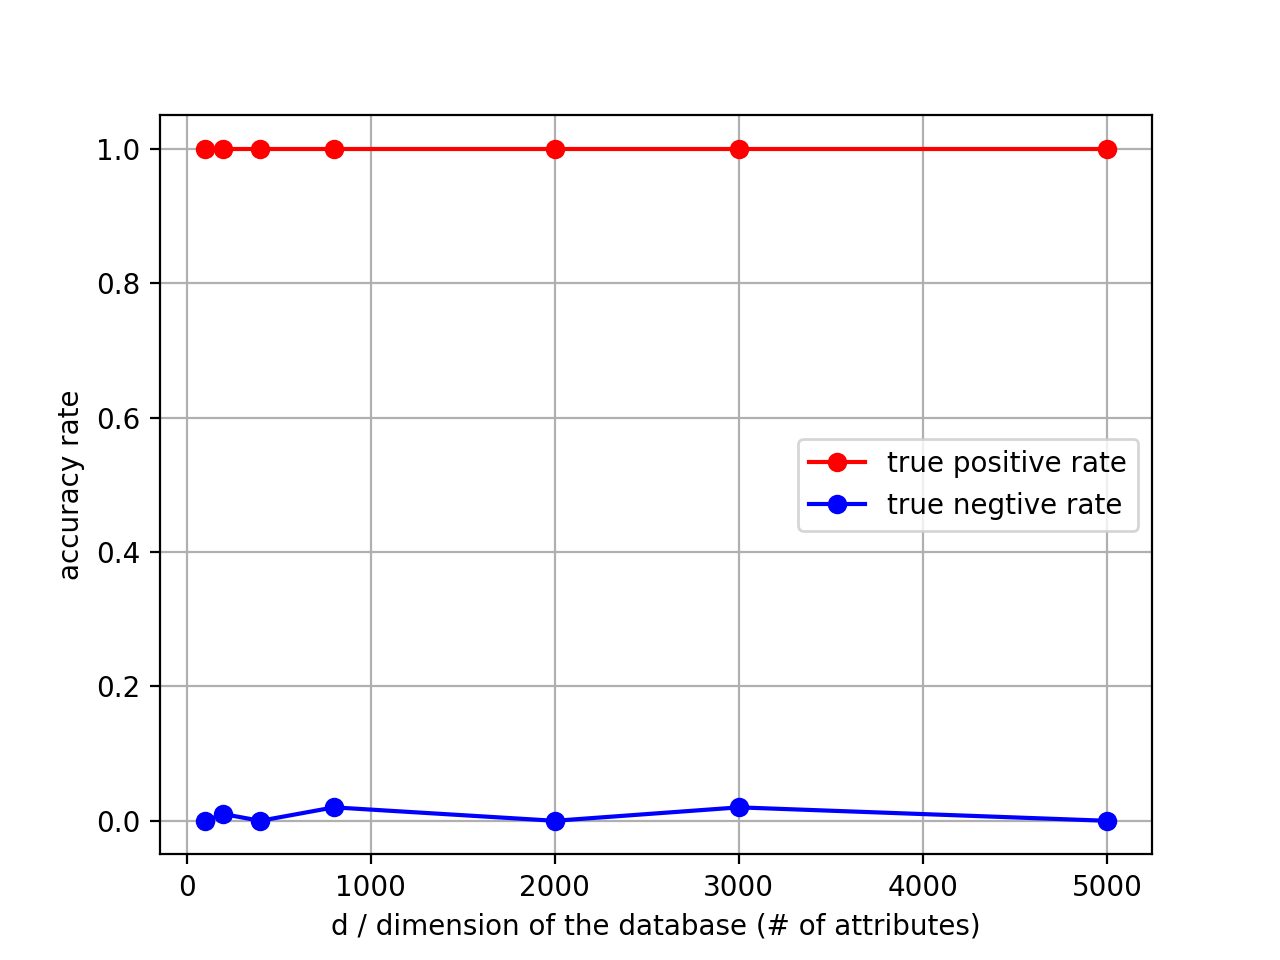
\includegraphics[width=0.5\textwidth]{p2-3.eps}
    \caption{P3: True Positive and True Negtive of Linear Regression Attack}
    \label{fig-p2-3}
\end{figure}
%	
	\item \textbf{Results Discussion}
	Close to perfect.
	\item \textbf{Code}
	See Appendix \ref{code-p2-3}


\end{itemize}
\end{enumerate}


\section{Problem 3}
\begin{enumerate}
	\item (reading)
	\item (Sampling)
	\begin{enumerate}
		\item 
		Given $S_i$ sampled from $a_1, \ldots, a_n$, we have:
		\[
		E(S_i) = \bar{a}.
		\]
		%
		Let $E(S) = E(\sum S_i) = k \bar{a}$, we have:
		%
		\[
		\begin{array}{ccl}
		Pr[error \leq \alpha] 
		& = & Pr[|\hat{S} - \bar{a}| \leq \alpha]\\
		%
		& = & Pr[|\frac{1}{k}\sum S_i - \bar{a}| \leq \alpha] = Pr[|\sum S_i - k\bar{a}| \leq k\alpha]\\
		%
		& = & Pr[|S - E(S)| \leq k\alpha]\\
		%
		& \geq & 1 - 2 \exp \big( 
		- \frac{\alpha^2 / \bar{a}^2}
		{2 + \alpha / \bar{a}} k \bar{a} \big)
		(\text{applying the Chernoff bounds})\\
		\end{array}
		\]
		%
		By guaranteeing $\delta = 2 \exp \big( 
		- \frac{\alpha^2 / \bar{a}^2}
		{2 + \alpha / \bar{a}} k \bar{a} \big)$, we have:
		%
		\[
		k = \frac{\ln(\frac{2}{\delta})(2 + \frac{\alpha}{\bar{a}})\bar{a}}
		{\alpha^2}
		\]
		%
		%
		\item
		let $\mu_i$ be the true proportion of individuals in the population who answer ``yes'' for function $f_i$, i.e. $\frac{1}{n}\sum_{j = 1}^{n}f_i(x_j) = \mu_i$. We know $E[f_i(S_j)] = \mu_i$ and $E[f_i(S)] = k\mu_i$. Let $f_i(S) = \sum_{j = 1}^{k}f_1(S_j)$, we have for all $f_i$:
		%
		\[
		\begin{array}{ccl}
		& & Pr[
		|\frac{1}{k}f_1(S) - \mu_1| 
		\leq \alpha 
		\land \ldots \land 
		|\frac{1}{k}f_d(S) - \mu_d| 
		\leq \alpha]\\
		& = & 1 - Pr[
		|\frac{1}{k}f_1(S) - \mu_1| 
		\geq \alpha  
		\lor \ldots \lor 
		|\frac{1}{k}f_d(S) - \mu_d|
		\geq \alpha] \\
		& = & 1 - Pr[
		|f_1(S) - k\mu_1| 
		\geq k\alpha  
		\lor \ldots \lor 
		|f_d(S) - k \mu_d|
		\geq k\alpha] \\
		%
		& \geq & 1 - \sum\limits_{i = 1}^{d} 
		Pr[|f_1(S) - k \mu_1| \geq k \alpha]
		%
		~~~~(\text{applying the union bound})\\
		%
		& \geq & 1 - 2 \sum\limits_{i = 1}^{d}
		\exp(- \frac{\alpha^2 / \mu_i}{ 2 + \alpha / \mu_i}
		k \mu_i) 
		%
		~~~~(\text{applying the Chernoff bound})\\
		%
		& = & 1 - 2 \sum\limits_{i = 1}^{d}
		\exp(- \frac{k \alpha^2}{ 2\mu_i + \alpha })\\
		%		
		& \geq & 1 - 2d\exp(- \frac{k \alpha^2}{ 2 + \alpha })
		\end{array}
		\] 
		%
		To guaranteeing the $\delta = 2d\exp(- \frac{k \alpha^2}{ 2 + \alpha })$, we have:
		%
		\[
		d = \frac{\ln(2d \frac{1}{\delta})(2 + \alpha)}
		{\alpha^2}
		= \frac{(\ln(2d) + \ln( \frac{1}{\delta}))(2 + \alpha)}
		{\alpha^2}
		= O(\frac{\ln(2d) + \ln( \frac{1}{\delta})}
		{\alpha^2})
		\]
		%
		%
		\item
		Given $err = \frac{Hamming(\hat{x}, x)}{n}$, i.e.
		% 
		$$err = \frac{1}{n}||\hat{x} - x||_{l_1} 
		= \frac{1}{n} \sum_{i = 1}^{n} |\hat{x}(i) - x(i)|$$
		%
		Let $x'$ be the sub data set which is not used to answer mechanism, and $\hat{x'}$ be the gauss of this subset.
		%
		The best the adversary can do is perfectly recover the subset used ($x \setminus x'$) and randomly guess $x'$, so we have:
		\[
		E(err)  = \frac{1}{n}( \frac{2 n}{3} E(|\hat{x'}(i) - x'(i)|) + \frac{n}{3} * 0) = \frac{1}{3}
		\]
		By applying the Chernoff bound, we have:
		\[
		Pr[err \geq (1 + \epsilon) \frac{1}{3}]
		\leq 1 - \exp(- \frac{\epsilon^2}{2 + \epsilon} \frac{n}{3})
		\]
		%
		Given $\Omega(n) \sim \exp(- \frac{\epsilon^2}{2 + \epsilon} \frac{n}{3})$, we have:
		%
		\[
		err \geq (1 + \epsilon) \frac{1}{3} \geq \frac{1}{3} > \frac{1}{4}
		\]

	\end{enumerate}
\end{enumerate}

\section{Problem 4}

\begin{enumerate}
	\item (Sample Size Calculations.)
\begin{enumerate}
	\item
	Given $X_i \sim Bernoulli(p)$, we have:
	\[
	E(X_i) = p, ~~ Var(X_i) = p(1 - p).
	\]
	Since $\bar{X}$ is the mean of i.i.d. $X_1, \cdots, X_n$, we have:
	\[
	E(\bar{X}) = p, ~~ Var(\bar{X}) = \frac{1}{n}p(1 - p).
	\]
	%
	To guarantee that variance of $\bar{X} < \alpha$, the following bound on n can be derived by:
	\[
	\begin{array}{ccc}
	Var(\bar{X}) = \frac{1}{n}p(1 - p)& < & \alpha\\
	n & > & \frac{p(1 - p)}{\alpha} ~ (\star).
	\end{array}
	\]
	%
	Then we have $n_{\epsilon}(\alpha, p)$ be the ceil of $(\star)$:
	\[
	n_{\epsilon}(\alpha, p) = \Bigg\lceil \frac{p(1-p)}{\alpha} \Bigg\rceil.
	\]
	%
	%
	%
	Given $A_{\epsilon}(X) = \bar{X} + Z$ where $Z \sim Lap(1/n\epsilon)$, we have:
	\[
	Var(A_{\epsilon}(X)) = Var(\bar{X}) + Var(Z) = \frac{1}{n}p(1 - p) + \frac{2}{(n\epsilon)^2}
	\]
	%
	Similarly, to guarantee that variance of $\bar{X} < \alpha$, the following bound on $n^*$ can be derived by:
	\[
	\begin{array}{ccc}
	Var(A_{\epsilon}(X)) = 
	\frac{1}{n}p(1 - p) + \frac{2}{(n\epsilon)^2} & < & \alpha\\
	n & > & \frac{p(1 - p)}{\alpha - \frac{2}{(n\epsilon)^2}} ~ (\diamond).
	\end{array}
	\]
	%
	Then we have $n_{\epsilon}(\alpha, p)$ be the ceil of $(\star)$:
	\[
	n^*_{\epsilon}(\alpha, p) 
	= \Bigg\lceil \frac{p(1-p)}{\alpha - \frac{2}{(n\epsilon)^2}} \Bigg\rceil
	\]
	%
	%
	%
	%
	%
	\item 
	%
	\[
	n_{\epsilon}(\alpha, p) - n^*_{\epsilon}(\alpha, p)
	= p(1-p)\big( \frac{1}{\alpha} - \frac{1}{\alpha - 2/(n\epsilon)^2} \big)
	\]
	%
	Since 
	\[
	\big( \frac{1}{\alpha} - \frac{1}{\alpha - 2/(n\epsilon)^2} \big)
	\left \{ 
	\begin{array}{lr}
	> 0 &  \alpha < \frac{1}{\alpha - 2/(n\epsilon)^2}\\
	%
	< 0 & \alpha > \frac{1}{\alpha - 2/(n\epsilon)^2}
	\end{array}
	\right \},
	\] 
	%
	we have the value of $n_{\epsilon}(\alpha, p) - n^*_{\epsilon}(\alpha, p)$:
	%
	\[
	\left \{ 
	\begin{array}{lr}
	\left \{
	\begin{array}{ll}
	\text{decrease} & p \in [0.5, 1]\\
	\text{increase} & p \in [0, 0.5)
	\end{array}
	\right \}
	&  \alpha < \frac{1}{\alpha - 2/(n\epsilon)^2}\\
	%
	\left \{
	\begin{array}{ll}
	\text{increase} & p \in [0.5, 1]\\
	\text{decrease} & p \in [0, 0.5)
	\end{array}
	\right \}
	& \alpha > \frac{1}{\alpha - 2/(n\epsilon)^2}
	\end{array}
	\right \},
	\] 
	
	%
	\item 
	%
	When $A_{\epsilon}$ is the $\epsilon$-DP randomized response estimator, we have:
	%
	\[
	q_{\epsilon}(X_i) = 
	\left\{
	\begin{array}{cc}
	X_i 	& w.p. ~ \frac{e^\epsilon}{1 + e^{\epsilon}} \\
	1 - X_i & w.p. ~ \frac{1}{1 + e^{\epsilon}}
	\end{array}\right \},
	%
	~
	A_{\epsilon}(X) = \frac{1}{n} \sum_{i} q_{\epsilon}(X_i)
	\]
	we have the expectation and variance for $q_{\epsilon}(X_i)$ as:
	\[
	\begin{array}{ll}
	E(q_{\epsilon}(X_i)) 
	& = E(\frac{e^\epsilon}{1 + e^{\epsilon}}X_i 
	+ \frac{1}{1 + e^{\epsilon}}(1 - X_i)) 
	= \frac{1}{1 + e^{\epsilon}}( (e^{\epsilon} - 1)E(X_i) + 1)
	= \frac{1}{1 + e^{\epsilon}}( (e^{\epsilon} - 1)p + 1)\\
	Var(q_{\epsilon}(X_i))
	& = E \big( (q_{\epsilon}(X_i) - E(q_{\epsilon}(X_i)) )^2 \big) 
	= E\big( 
	\frac{e^\epsilon}{1 + e^{\epsilon}}
	\big(X_i - E(q_{\epsilon}(X_i)) \big)^2
	+
	\frac{1}{1 + e^{\epsilon}}
	\big((1 - X_i) - E(q_{\epsilon}(X_i)) \big)^2
	\big)
	\end{array}
	\]
	Let $E_{q_{\epsilon}} = E(q_{\epsilon}(X_i))$, we have:
	\[
	\begin{array}{ll}
	Var(q_{\epsilon}(X_i))
	& = \frac{1}{1 + e^{\epsilon}}
	E((1 + e^{\epsilon})(X_i^2 + E_{q_{\epsilon}}^2)
	+ 1 - 2E_{q_{\epsilon}} + 2(1 - e^{\epsilon})X_iE_{q_{\epsilon}})\\
	%
	& = (p + E_{q_{\epsilon}}^2) + \frac{1}{1 + e^{\epsilon}}(1 - 2E_{q_{\epsilon}} + 2(1 - e^{\epsilon})pE_{q_{\epsilon}})\\
	%
	& = (\frac{1}{1 + e^{\epsilon}} + p - E_{q_{\epsilon}}^2)
	\end{array}
	\]
	Then we have:
	\[
	\begin{array}{ll}
	E(A_{\epsilon}(X))
	& = E\big(
	\frac{1}{n} \sum_{i} q_{\epsilon}(X_i)
	\big) 
	= \frac{1}{1 + e^{\epsilon}}( (e^{\epsilon} - 1)p + 1)\\
	Var(A_{\epsilon}(X))
	& = \frac{1}{n} Var\big( q_{\epsilon}(X_i) \big) \big) 
	= \frac{1}{n}
	(\frac{1}{1 + e^{\epsilon}} + p - E_{q_{\epsilon}}^2)
	\end{array}
	\]
	%
	To guarantee $Var(A_{\epsilon}(X)) > \alpha$, we have:
	\[
	n^*_{\alpha, p} > 
	\frac{\frac{1}{1 + e^{\epsilon}} + p - E_{q_{\epsilon}}^2}
		 {\alpha}
	\]



\end{enumerate}

\item (Global Sensitivities.)
\begin{enumerate}
	\item $1.0$
	\item $1.0$
	\item $\frac{1}{n}$
	\item $1.0$
	\item $(n - 1)$, where $n$ is the size of the Census data (n is not explicitely noted).
	\item $1.0$
	\item $\infty$
	\item $1.0$
\end{enumerate}
\item (Amplification by subsampling)
$B_{p, \epsilon}$ is $\ln(1 + (e^{\epsilon} - 1)p)$-differentially private.
\begin{proof}
Given $A_{\epsilon}$ is $\epsilon$-DP, we have for arbitrary adjacent data set $x$, $x'$ and $G$ be the subset of output domain:
\[
	e^{-\epsilon} \leq 
	\frac{Pr[A_{\epsilon}(x) \in G]}{Pr[A_{\epsilon}(x') \in G]} 
	\leq e^{\epsilon}
\]
So we have for $B_{p, \epsilon}$ under the same setting where $x, x'$ differ in $x_k$ and $S$ is the subset:
\[
\begin{array}{ccc}
	\frac{Pr[B_{p, \epsilon}(x') \in G]}
	{Pr[B_{p, \epsilon}(x) \in G]}
	%
	& = & 
	\frac{Pr[A_{\epsilon}(S) \in G \land x_k \notin S  
	\cup A_{\epsilon}(S') \in G \land x_k \in S]}
	{Pr[A_{\epsilon}(S) \in G]}
	\\
	%
	& \leq &
	\frac{Pr[A_{\epsilon}(S) \in G \land x_k \notin S]
	+ Pr[A_{\epsilon}(S') \in G \land x_k \in S]}
	{Pr[A_{\epsilon}(S) \in G]}
	\\
	%
	& = &
	\frac{(1 - p)Pr[A_{\epsilon}(S) \in G]
	+ p Pr[A_{\epsilon}(S') \in G]}
	{Pr[A_{\epsilon}(S) \in G]}
	\\
	%
	& \leq &
	\frac{(1 - p)Pr[A_{\epsilon}(S) \in G]
	+ p e^{\epsilon}Pr[A_{\epsilon}(S) \in G]}
	{Pr[A_{\epsilon}(S) \in G]}
	\\
	%
	& = & 1 + (e^{\epsilon} - 1)p
\end{array}
\]
The other side can be proved trivially. Then we have $B_{p, \epsilon}$ is $\ln(1 + (e^{\epsilon} - 1)p)$-DP.

\end{proof}
%
%
\item (K-means algorithm)
\begin{itemize}
\item \textbf{Algorithm Description}
%
The algorithm is the same as algorithm presented in class
%
\begin{algorithm}
\caption{Differentially Private K-means}
\label{alg_p4-3}
\begin{algorithmic}
\REQUIRE The rows and columns of the data points $n, d$, the parameters $k, T, \epsilon$, Centers $M$ and parameter $\sigma$ for generating data points.
\STATE {\bf Generate data points $x_i = M + (z \leftarrow N(0, \sigma)^d)$}
\STATE  {\bf let}\ $k = M.length$, $\epsilon' = \frac{\epsilon}{2T}$.  
\STATE  {\bf Initialize}\ $c$ randomly from $[-1, 1]^{d \times k}$. 
\STATE 	{\bf For}\ $t \in [T]$  {\bf do}.
\STATE \qquad	$s_j = \{i : c_j$ is the closet center to $x_i \}$.
\STATE \qquad	$n_j = |s_j| + Lap(\frac{1}{\epsilon'})$ 
\STATE \qquad	$a_j = \sum_{i \in s_j}x_i
			+ Lap(\frac{2}{\epsilon'})^d$ 
\STATE \qquad	$c_j^t = \frac{a_j}{n_j}$ if $n_j > 5$ else randomly from $[-1, 1]^{d \times k}$.
		
\RETURN $c$.
\end{algorithmic}
\end{algorithm}

%
\item \textbf{Experimental Results Plotting}
%
Figrue \ref{fig-p4-3}.
		\begin{figure*}[t!]
		    \centering
		    \begin{subfigure}[t]{0.5\textwidth}
		        \centering
		        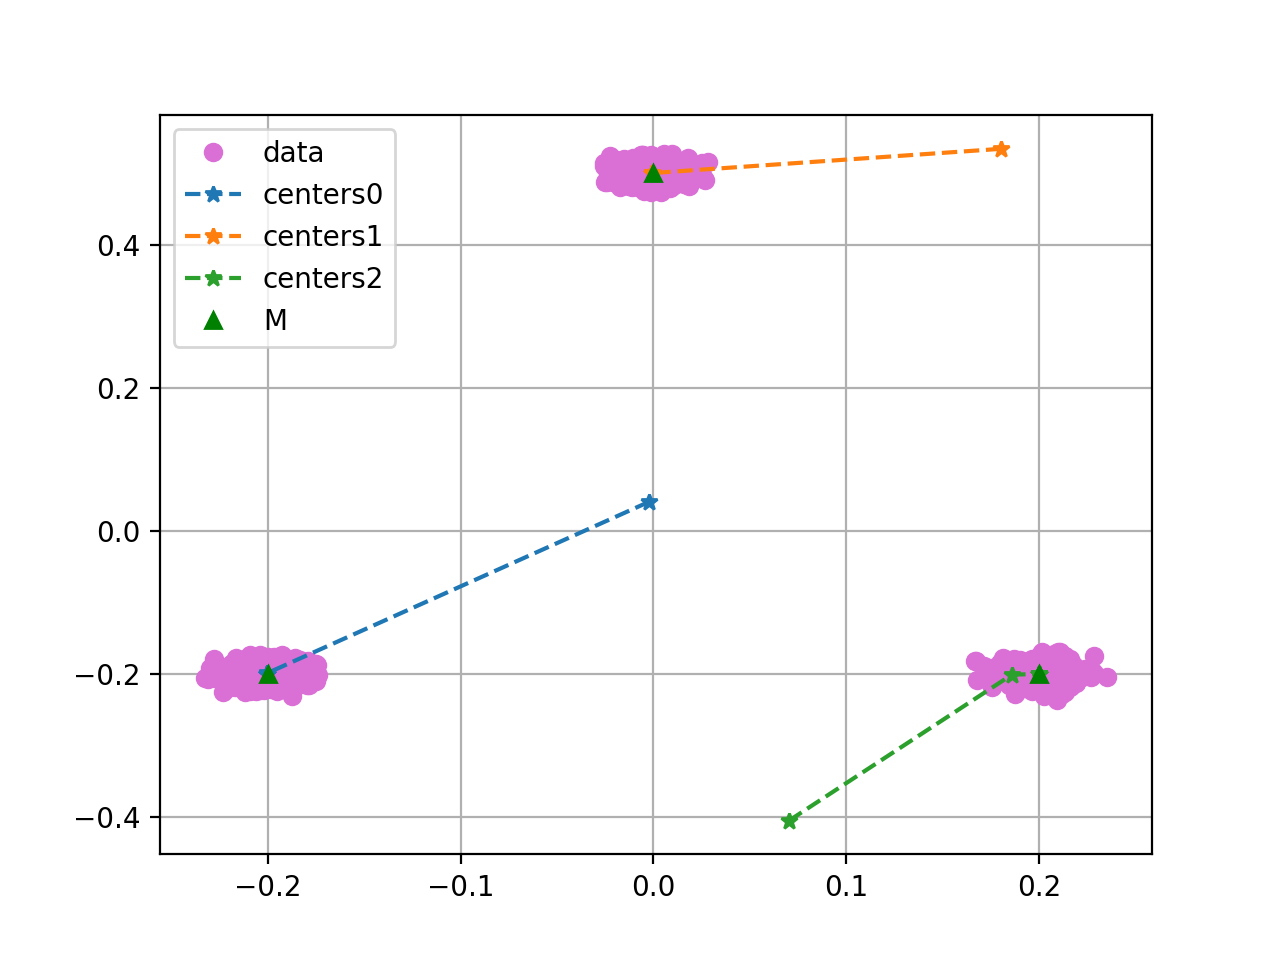
\includegraphics[width=\textwidth]{p4-3a.eps}
		        \caption{Pure K-Means}
		    \end{subfigure}%
		    ~ 
		    \begin{subfigure}[t]{0.5\textwidth}
		        \centering
		        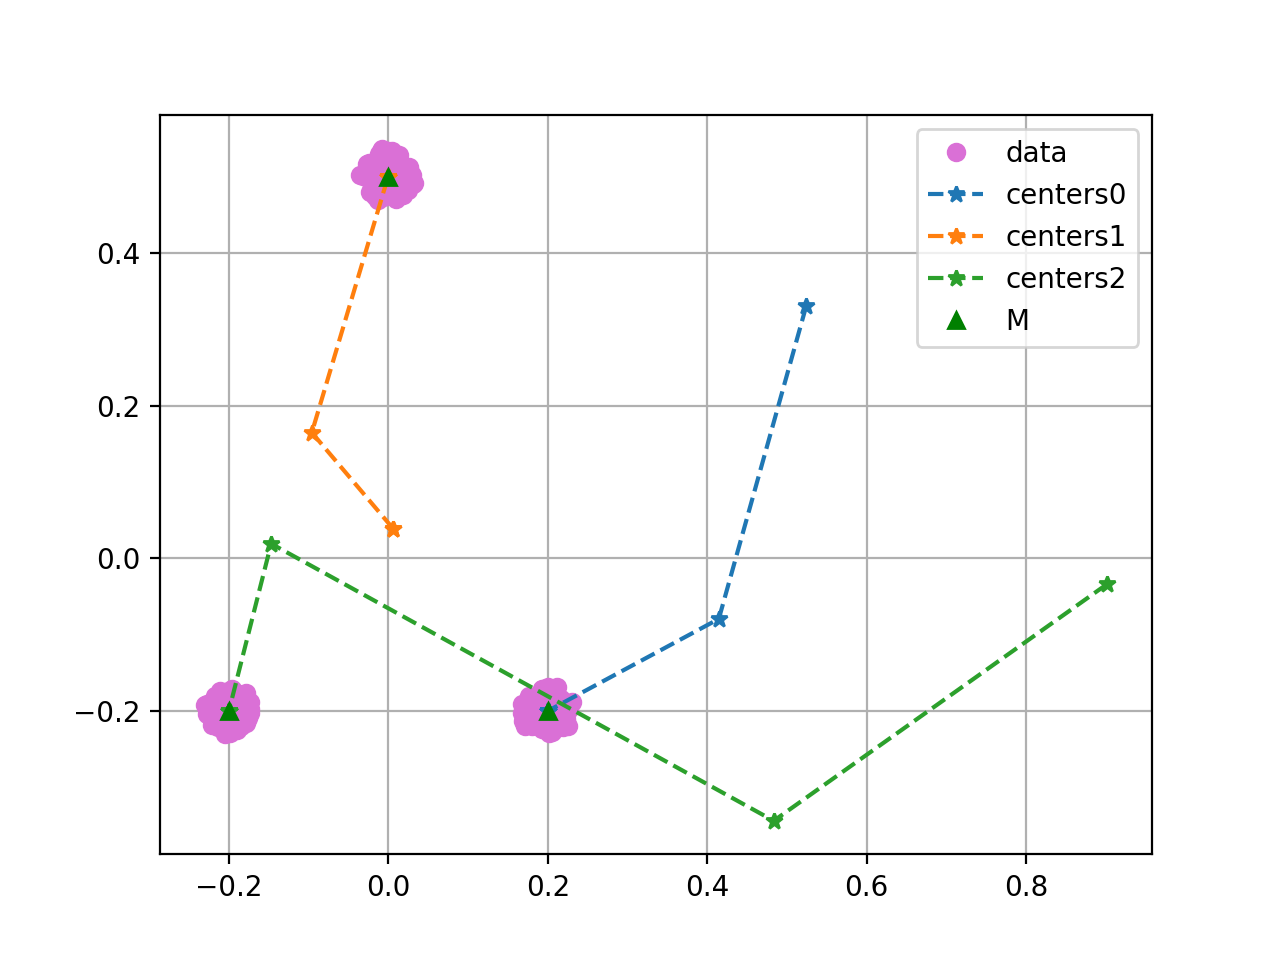
\includegraphics[width=\textwidth]{p4-3b.eps}
		        \caption{Private K-Means}
		    \end{subfigure}
		    \caption{P4: K-Means Algorithms}
		    \label{fig-p4-3}
		\end{figure*}
%
\item \textbf{Results Discussion}
%
The results are shown in Fig. \ref{fig-p4-3}. 
%
\\
%
\textbf{In Fig. \ref{fig-p4-3}(a)}, I firstly implemented the pure k-means algorithm which performs very well with only $2$ or even $1$ iteration arrived the true center.
%
\\
%
Then \textbf{in Fig. \ref{fig-p4-3}(b)}, the differentially private k-means algorithm performs also good but with few more iteration in order to arrive the true center.
%
\\
%
During my experiments, some times the algorithm doesn't converge to a final center because of the randomness. 

\item \textbf{Code Documentation}
See Appendix \ref{code-p4-3}
%

\end{itemize}

\end{enumerate}

\section*{Appendix}

\begin{lstlisting}[label=code-alg2, language=Python, caption=Python Code For Algorithm 2 Simple Histogram CDF]
import numpy as np
import matplotlib.pyplot as plt
import math

#############################################################################
#GENERATING DATA SIZE AND CONRRESPONDING PARAMETER
#############################################################################

def gen_dataset(n):
	data = []
	for _ in range(n):
		x = np.random.normal(0.7, 0.01)
		data.append(0.0 if x < 0.0 else 0.99 if x > 1.0 else x)

	return np.array(data)

def gen_datasizes(r, step):
	return [i*step for i in range(r[0]/step,r[1]/step + 1)]

#############################################################################
#SETTING UP THE GRANULARITY OF T
#############################################################################

def gen_t():
	return [0.1 * i for i in range(10)]

#############################################################################
#SIMPLE HISTOGRAM ALGORITHM
#############################################################################
def Simple_Histogram(x, a, eps):
	Y = [0]
	n = len(x)
	for j in range(1, int(1/a) + 1):
		I0, I1 = (j - 1) * a, j * a
		count = 0
		for xi in x:
			count += 1 if (xi < I1 and xi >= I0) else 0.0
		Y.append(count/n + np.random.laplace(0.0, 2/(eps * n)))
	return Y

#############################################################################
#SIMPLE HISTOGRAM CDF ALGORITHM
#############################################################################
def Simple_Histogram_CDF(x, a, eps):
	Y = Y = Simple_Histogram(x, a, eps)
	n = len(x)
	def eCDF(t):
		return sum([Y[j] for j in range(1, int(math.floor(t/a)))]) + (t/a - math.floor(t/a)) * Y[int(math.floor(t/a)) + 1]
	
	ecdf = np.array([eCDF(t) for t in gen_t()])

	return Y, ecdf

#############################################################################
# CDF FUNCTION
#############################################################################
def CDF(x):
	n = len(x)
	def CDFt(t):
		count = 0.0
		for xi in x:
			if xi < t: count += 1.0
		return count/n
	return np.array([CDFt(t) for t in gen_t()])


#############################################################################
# ERROR COMPUTING
def error(cdf, ecdf):
	return max(abs(cdf - ecdf))

#############################################################################
# TEST SIMPLE OR TREE CDF FUNCTION
def expermt(eps, n, a):
	e = 0.0
	for _ in range(20):
		x = gen_dataset(n)
		Y, ecdf = Simple_Histogram_CDF(x, a, eps)
		cdf = CDF(x)
		e += error(cdf, ecdf)
	print a, e
	return e/20.0

def expermt_va(eps, n, va):
	return [expermt(eps, n, a) for a in va]

def plot_accuracy(ys, ns):
	plt.figure()
	plt.plot(ns, ys, "ro-", label = "Error")
	plt.xlabel(r'$\alpha = \frac{1}{2^{x}}$')
	plt.ylabel("Error")
	plt.title(r"Simple Histogram CDF with n = $10^5$")
	plt.legend()
	plt.grid()
	plt.show()

if __name__ == "__main__":
	#############################################################################
	#SETTING UP THE PARAMETERS WHEN DOING GROUPS EXPERIMENTS
	#############################################################################
	eps = 0.5
	n = 100000
	va = [(1.0/2) ** i for i in range(1, 16)]
	plot_accuracy(expermt_va(eps, n, va), range(1, 16))

\end{lstlisting}

\begin{lstlisting}[label=code-alg3, language=Python, caption=Python Code For Algorithm 2 Tree Histogram CDF]
import numpy as np
import matplotlib.pyplot as plt
import math

#############################################################################
#GENERATING DATA SIZE AND CONRRESPONDING PARAMETER
#############################################################################

def gen_dataset(n):
	data = []
	for _ in range(n):
		x = np.random.normal(0.7, 0.01)
		data.append(0.0 if x < 0.0 else 0.99 if x > 1.0 else x)

	return np.array(data)

def gen_datasizes(r, step):
	return [i*step for i in range(r[0]/step,r[1]/step + 1)]

#############################################################################
#SETTING UP THE GRANULARITY OF T
#############################################################################

def gen_t():
	return [0.1 * i for i in range(10)]


#############################################################################
#SIMPLE HISTOGRAM ALGORITHM
#############################################################################
def Simple_Histogram(x, a, eps):
	Y = [0]
	n = len(x)
	for j in range(1, int(1/a) + 1):
		I0, I1 = (j - 1) * a, j * a
		count = 0
		for xi in x:
			count += 1 if (xi < I1 and xi >= I0) else 0.0
		Y.append(count/n + np.random.laplace(0.0, 2/(eps * n)))
	return Y



#############################################################################
#TREE HISTOGRAM CDF ALGORITHM
#############################################################################
def Tree_Histogram_CDF(x, eps, l):
	va = [(1.0/2) ** i for i in range(1, l)]
	vY = [ Simple_Histogram(x, a, eps) for a in va]
	def eCDF(t):
		d = np.argmin(np.array([(t/a - math.floor(t/a)) for a in va]))
		Y, a = vY[d], va[d]
		return sum([Y[j] for j in range(1, int(math.floor(t/a)))]) + (t/a - math.floor(t/a)) * Y[int(math.floor(t/a)) + 1]
	ecdf = np.array([eCDF(t) for t in gen_t()])

	return ecdf

#############################################################################
# CDF FUNCTION
#############################################################################
def CDF(x):
	n = len(x)
	def CDFt(t):
		count = 0.0
		for xi in x:
			if xi < t: count += 1.0
		return count/n
	return np.array([CDFt(t) for t in gen_t()])


#############################################################################
# ERROR COMPUTING
def error(cdf, ecdf):
	return max(abs(cdf - ecdf))

#############################################################################
# TEST SIMPLE OR TREE CDF FUNCTION
def expermt(eps, n, a):
	e = 0.0
	for _ in range(20):
		x = gen_dataset(n)
		Y, ecdf = Tree_Histogram_CDF(x, a, eps)
		cdf = CDF(x)
		e += error(cdf, ecdf)
	print a, e
	return e/20.0

def expermt_va(eps, n, va):
	return [expermt(eps, n, a) for a in va]

def plot_accuracy(ys, ns):
	plt.figure()
	plt.plot(ns, ys, "ro-", label = "Error")
	plt.xlabel(r'$\alpha = \frac{1}{2^{x}}$')
	plt.ylabel("Error")
	plt.title(r"Tree Histogram CDF with n = $10^3$")
	plt.legend()
	plt.grid()
	plt.show()

if __name__ == "__main__":
	##############################################################
	#SETTING UP THE PARAMETERS WHEN DOING GROUPS EXPERIMENTS
	#############################################################
	eps = 0.5
	n = 1000
	vl = range(1, 16)
	plot_accuracy(expermt_va(eps, n, va), range(1, 16))

\end{lstlisting}





\end{document}
